\chapter{Potenciais termodinâmicos}\label{ch:b2:thermodynamic-potentials}

Estique depressa um elástico e encoste-o no lábio: ele está quente;
deixe-o contrair e ele está frio. Pendure um peso nele e aqueça-o com um
secador de cabelo: ele \emph{encurta}. Nenhuma mola de aço se comporta assim, e a
razão é que a tensão de um elástico não é questão de energia, mas de
entropia --- as cadeias esticadas têm menos maneiras de se arranjar.
Para raciocinar sobre essas coisas é preciso saber o que um sistema a
temperatura fixa, ou a temperatura e pressão fixas, tende a fazer, e
quanto trabalho se pode extrair dele: perguntas que a energia interna e
a entropia respondem apenas desajeitadamente, porque falam a língua de um
sistema isolado. Este capítulo introduz as duas funções construídas para
as condições do laboratório, a \emph{\omterm{def:b2:thermodynamic-potentials:FG}{energia livre} de Helmholtz} $F = U -
TS$ e a \emph{\omterm{def:b2:thermodynamic-potentials:FG}{entalpia livre} de Gibbs} $G = H - TS$, mostra que elas
medem o trabalho recuperável e decrescem rumo ao equilíbrio, extrai
de seus diferenciais as relações de Maxwell que ligam grandezas
que ninguém julgaria aparentadas, e aplica tudo isso ao
equilíbrio de duas fases, em que $G$ decide qual fase vence e
devolve a fórmula de Clapeyron.

\begin{omfigure}
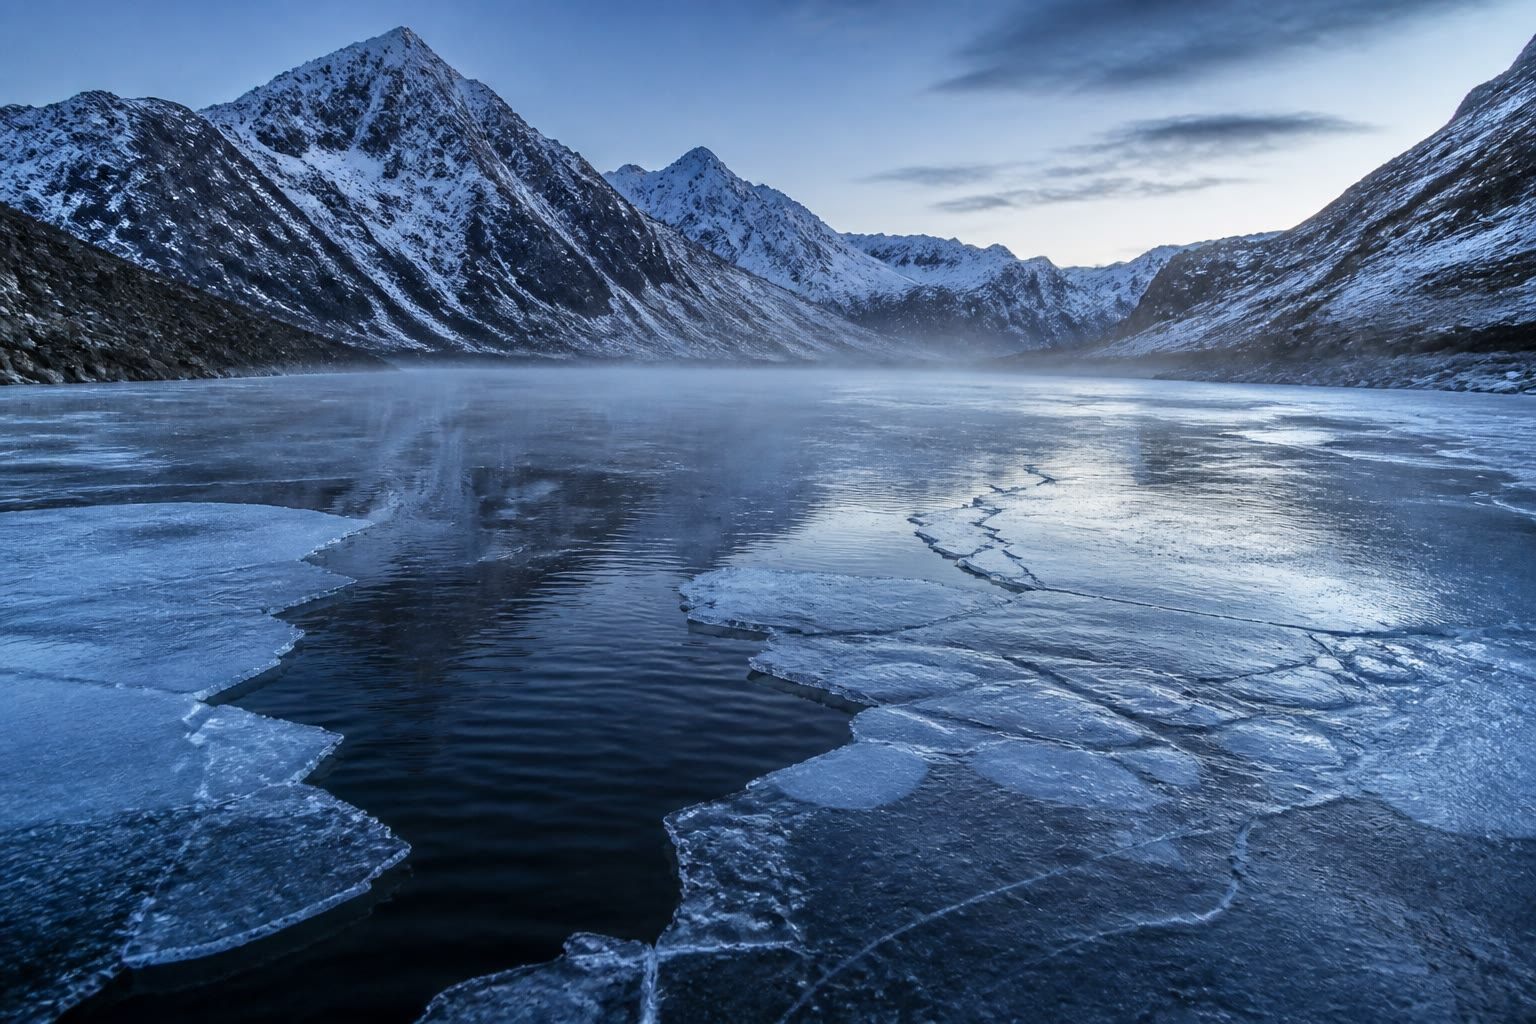
\includegraphics[width=0.58\linewidth]{images/book4/ai/b4-28-ice-lake-dawn.jpg}

{\small Gelo e água coexistindo num lago ao amanhecer: no ponto de
fusão as duas fases têm a mesma \omterm{def:b2:thermodynamic-potentials:FG}{entalpia livre} por quilograma, e uma
pequena mudança de pressão ou de temperatura desequilibra a balança --- a
inclinação de Clapeyron diz de quanto.}
\end{omfigure}

\section{A identidade fundamental e suas variáveis}

\begin{proposition}[Identidade fundamental]\label{prop:b2:thermodynamic-potentials:identity}
Para um sistema fechado de composição fixa, a energia interna,
vista como função da entropia e do volume, satisfaz
\[
\dd U = T\,\dd S - P\,\dd V, \qquad
T = \Big(\frac{\partial U}{\partial S}\Big)_V, \quad
P = -\Big(\frac{\partial U}{\partial V}\Big)_S ,
\]
e a \omterm{thm:b2:open-systems:firstlaw}{entalpia} $H = U + PV$ satisfaz $\dd H = T\,\dd S + V\,\dd P$.
Cada função, em suas \emph{variáveis naturais}\index{variáveis
naturais} --- $(S,V)$ para $U$, $(S,P)$ para $H$ --- contém toda a
termodinâmica do sistema: suas derivadas parciais dão as demais
variáveis de estado. O segundo princípio seleciona o equilíbrio de um sistema
isolado ($U$, $V$ fixos) como o estado de $S$ máxima.
\end{proposition}

\begin{proof}
O primeiro princípio para uma transformação reversível, $\dd U = \delta Q_{\text{rev}}
+ \delta W_{\text{rev}} = T\,\dd S - P\,\dd V$, envolve apenas funções de
estado e portanto vale para qualquer variação infinitesimal entre
estados de equilíbrio. Acrescente $\dd(PV)$ para $H$.
\end{proof}

\begin{remark}[Por que novas funções]\label{rem:b2:thermodynamic-potentials:why}
As experiências não são feitas a entropia fixa. O balão de um químico fica à
temperatura da sala e à pressão da atmosfera; um
pistão num termostato trabalha a $T$ fixo. Queremos funções cujas
\omterm{prop:b2:thermodynamic-potentials:identity}{variáveis naturais} sejam $(T,V)$ e $(T,P)$, e que desempenhem, nessas
condições, o papel que $S$ desempenha para um sistema isolado: dizer
para que lado o sistema evolui e quanto trabalho ele pode fornecer. Uma
\emph{transformada de Legendre} --- subtrair $TS$ para trocar $S$ por $T$ como
variável independente --- as constrói.
\end{remark}

\section{Energia livre e entalpia livre}

\begin{definition}[Energia livre de Helmholtz, entalpia livre de Gibbs]\label{def:b2:thermodynamic-potentials:FG}
\[
F = U - TS \quad\text{(\emph{energia livre}\index{energia livre})}, \qquad
G = H - TS = U + PV - TS \quad\text{(\emph{entalpia livre}\index{entalpia livre})}.
\]
Ambas são funções de estado extensivas, medidas em joules.
\end{definition}

\begin{theorem}[Diferenciais e grandezas derivadas]\label{thm:b2:thermodynamic-potentials:dFdG}
\[
\dd F = -S\,\dd T - P\,\dd V, \qquad
\dd G = -S\,\dd T + V\,\dd P ;
\]
e daí, nas \omterm{prop:b2:thermodynamic-potentials:identity}{variáveis naturais} $(T,V)$ de $F$ e $(T,P)$ de $G$,
\[
S = -\Big(\frac{\partial F}{\partial T}\Big)_V, \quad
P = -\Big(\frac{\partial F}{\partial V}\Big)_T, \qquad
S = -\Big(\frac{\partial G}{\partial T}\Big)_P, \quad
V = \Big(\frac{\partial G}{\partial P}\Big)_T ,
\]
e (Gibbs--Helmholtz) $U = F - T(\partial F/\partial T)_V =
-T^2\,\partial(F/T)/\partial T$, $H = -T^2\,\partial(G/T)/\partial T$.
Conhecer $F(T,V)$ ou $G(T,P)$ é conhecer tudo: a equação de
estado, a entropia, a energia, as capacidades térmicas.
\end{theorem}

\begin{proof}
$\dd F = \dd U - T\dd S - S\dd T = -S\dd T - P\dd V$; do mesmo modo para $G$
a partir de $\dd H$. Leia as derivadas parciais; para Gibbs--Helmholtz,
$F - T\,\partial_TF = F + TS = U$ e $\partial_T(F/T) = (T\partial_TF -
F)/T^2 = -U/T^2$.
\end{proof}

\begin{example}[O gás perfeito]\label{ex:b2:thermodynamic-potentials:perfect}
Para $n$ mols, $U = nc_{V}T + U_0$ e $S = nc_V\ln T + nR\ln V + S_0$
dão $F(T,V) = -nRT\ln V + f(T)$: então $P = -\partial_VF = nRT/V$
--- a equação de estado sai de $F$ --- e $S = -\partial_TF$
devolve a entropia. Nas variáveis $(T,P)$, $G(T,P) = nRT\ln P +
g(T)$, de modo que $V = \partial_PG = nRT/P$, e a \omterm{def:b2:thermodynamic-potentials:FG}{entalpia livre} \emph{molar}
$\mu(T,P) = \mu^\circ(T) + RT\ln(P/P^\circ)$ --- o \emph{potencial
químico}\index{potencial químico} do gás, que cresce com sua
pressão: o gás escoa do $\mu$ alto para o baixo, aqui da pressão alta para a
baixa.
\end{example}

\section{Trabalho máximo e sentido da evolução}

\begin{theorem}[Transformações monotérmicas]\label{thm:b2:thermodynamic-potentials:monothermal}
Um sistema que troca calor com um único termostato a $T_0$, e cujas
temperaturas inicial e final valem $T_0$, recebe durante qualquer
transformação o trabalho
\[
W \ge \Delta F , \qquad\text{i.e.}\qquad W_{\text{recuperado}} = -W \le -\Delta F :
\]
a diminuição de $F$ é o \emph{trabalho máximo recuperável} do
sistema a temperatura fixa (atingido para uma transformação reversível) ---
daí energia ``livre'': a parte de $U$ que pode virar trabalho, sendo o
resto, $TS$, ligado. Se além disso a transformação for monobárica
(pressão $P_0$ do lado de fora, pressões inicial e final iguais a $P_0$), o trabalho
\emph{que não o da atmosfera} (\omterm{def:b2:open-systems:cv}{trabalho útil}, por exemplo elétrico)
satisfaz $W_{\text{u}} \ge \Delta G$: $-\Delta G$ é o \omterm{def:b2:open-systems:cv}{trabalho útil} máximo
recuperável a $T$ e $P$ fixos (o trabalho de uma célula a combustível, de uma
bateria).
\end{theorem}

\begin{proof}
Primeiro princípio: $\Delta U = W + Q$. Segundo princípio com um termostato: $\Delta S
= Q/T_0 + S_{\text{c}}$, $S_{\text{c}} \ge 0$, logo $Q \le T_0\Delta S$. Portanto
$W = \Delta U - Q \ge \Delta U - T_0\Delta S = \Delta(U - T_0S) = \Delta F$, usando
$T = T_0$ nas duas extremidades. Separando o trabalho da atmosfera $-P_0\Delta V$,
$W = W_{\text{u}} - P_0\Delta V$ e $W_{\text{u}} \ge \Delta U + P_0
\Delta V - T_0\Delta S = \Delta G$.
\end{proof}

\begin{theorem}[Critérios de evolução e de equilíbrio]\label{thm:b2:thermodynamic-potentials:criteria}
Um sistema mantido a $T$ e $V$ fixos e que não recebe trabalho só pode
evoluir de modo que \emph{$F$ diminua}; seu equilíbrio é o estado de
$F$ mínima. Um sistema mantido a $T$ e $P$ fixos e que não recebe \omterm{def:b2:open-systems:cv}{trabalho
útil} só pode evoluir de modo que \emph{$G$ diminua}; seu equilíbrio é
o estado de $G$ mínima. (Mais geralmente, para um sistema em contato com
um meio a $T_0$, $P_0$, a grandeza $U - T_0S + P_0V$ diminui.)
\end{theorem}

\begin{proof}
Tome $W = 0$ (resp.\ $W_{\text{u}} = 0$) no teorema anterior: $\Delta F
\le 0$ (resp.\ $\Delta G \le 0$), com igualdade para uma evolução reversível,
isto é, de equilíbrio.
\end{proof}

\begin{example}[Expansão isotérmica, real e ideal]\label{ex:b2:thermodynamic-potentials:expansion}
Um mol de gás a \qty{300}{K} se expande de \qty{1}{L} a \qty{10}{L} em
contato com o termostato: $\Delta F = -RT\ln 10 = \qty{-5.7}{kJ}$. Uma
expansão reversível recupera \qty{5.7}{kJ}; uma expansão contra a
atmosfera a \qty{1}{bar} recupera apenas $P_0\Delta V = \qty{0.9}{kJ}$; uma
expansão livre no vácuo, nada. Os \qty{5.7}{kJ} são o máximo que
o gás e seu termostato podem dar para essa mudança de estado, por mais
engenhosa que seja a máquina.
\end{example}

\section{As relações de Maxwell}

\begin{theorem}[Relações de Maxwell]\label{thm:b2:thermodynamic-potentials:maxwell}
Como $\dd F$ e $\dd G$ são diferenciais exatas (teorema de Schwarz
sobre as derivadas segundas mistas),
\[
\Big(\frac{\partial S}{\partial V}\Big)_T = \Big(\frac{\partial P}{\partial T}\Big)_V,
\qquad
\Big(\frac{\partial S}{\partial P}\Big)_T = -\Big(\frac{\partial V}{\partial T}\Big)_P .
\]
Elas exprimem o inatingível (como a entropia varia com o volume ou
a pressão a temperatura fixa) através da equação de estado. Duas
consequências:
\[
\Big(\frac{\partial U}{\partial V}\Big)_T = T\Big(\frac{\partial P}{\partial T}\Big)_V - P,
\qquad
C_P - C_V = T\Big(\frac{\partial P}{\partial T}\Big)_V\Big(\frac{\partial V}{\partial T}\Big)_P
= \frac{TV\alpha^2}{\kappa_T} ,
\]
com $\alpha = V^{-1}(\partial V/\partial T)_P$ o coeficiente de dilatação e
$\kappa_T = -V^{-1}(\partial V/\partial P)_T$ a compressibilidade isotérmica.
\end{theorem}

\begin{proof}
$\partial^2F/\partial T\partial V$ calculada nas duas ordens: $-\partial_VS =
-\partial_TP$. O mesmo para $G$. Depois $\dd U = T\dd S - P\dd V$ a $T$ fixo
dá $(\partial_VU)_T = T(\partial_VS)_T - P$; e $C_P - C_V$ segue
de escrever $S(T,V(T,P))$: $(\partial_TS)_P = (\partial_TS)_V +
(\partial_VS)_T(\partial_TV)_P$, multiplicado por $T$.
\end{proof}

\begin{example}[O que as relações revelam]\label{ex:b2:thermodynamic-potentials:reveal}
Para um gás perfeito, $T(\partial_TP)_V - P = 0$: a energia não depende
do volume (a lei de Joule reencontrada) e $C_P - C_V = nR$. Para um gás de van
der Waals, $(\partial_VU)_T = a/V_{\text{m}}^2$: a pressão interna das
atrações. Para a água líquida, $(\partial_TP)_V = \alpha/\kappa_T = 2.1
\times 10^{-4}/4.6 \times 10^{-10} = \qty{4.6e5}{Pa/K}$: aquecer água num
recipiente rígido e cheio de um kelvin eleva a pressão de \qty{4.6}{bar}
(nunca vede uma garrafa cheia), e $(\partial_VU)_T \approx \qty{1400}{bar}$ ---
a coesão do líquido; e no entanto $c_P - c_V = Tv\alpha^2/\kappa_T \approx
\qty{30}{J/kg/K}$, menos de $1\%$ de $c_P$: para a matéria condensada as duas
capacidades térmicas quase coincidem.
\end{example}

\begin{proposition}[Elasticidade entrópica da borracha]\label{prop:b2:thermodynamic-potentials:rubber}
Para uma tira de comprimento $L$ sob a tensão $f$, $\dd U = T\dd S + f\dd L$
e $\dd F = -S\dd T + f\dd L$, de modo que $(\partial S/\partial L)_T =
-(\partial f/\partial T)_L$ e $(\partial U/\partial L)_T = f - T(\partial f/
\partial T)_L$. A borracha obedece, com boa aproximação, a $f = T\,\varphi(L)$
com $\varphi > 0$ para $L > L_0$: então $(\partial U/\partial L)_T = 0$ --- a
energia não muda ao esticar --- e $(\partial S/\partial L)_T =
-\varphi(L) < 0$: a tensão é \emph{entrópica}, $f = -T(\partial S/\partial
L)_T$, e a tira puxa de volta porque suas cadeias esticadas têm menos
configurações. Consequências: esticada isotermicamente ela cede calor
($Q = T\Delta S < 0$); esticada adiabaticamente ela esquenta; aquecida sob
carga constante ela se contrai ($f/T$ fixo significa $\varphi(L)$ fixo, de modo que a
$f$ fixo $\varphi$ deve cair quando $T$ sobe).
\end{proposition}

\begin{proof}
Relação de Maxwell a partir de $\dd F$; o resto é substituição. A
origem microscópica é o passeio aleatório do \cref{ch:b2:particle-diffusion}:
uma cadeia de $N$ elos de comprimento $a$ tem sua distância entre extremidades
distribuída como uma gaussiana de variância $Na^2$, de modo que o número de
configurações com extensão $L$ vale $\Omega \propto \eu^{-L^2/2Na^2}$, $S = S_0 -
k_BL^2/2Na^2$ e $f = k_BTL/Na^2$: uma mola cuja rigidez é
\emph{proporcional à temperatura}.
\end{proof}

\begin{omfigure}
\begin{tikzpicture}
  \begin{axis}[omaxis, width=6.2cm, height=4.4cm, xmin=0, xmax=400, ymin=0, ymax=1.25,
    xlabel={$T$ (\unit{K})}, ylabel={$f$ (un. arb.)}, xtick={100,200,300}, ytick=\empty, clip=false]
    \addplot[omDef, thick, domain=0:380] {x/300};
    \addplot[omDef, thick, domain=0:380] {0.6*x/300};
    \node[font=\scriptsize, omDef, anchor=west] at (axis cs:300,1.05) {$L - L_0$ grande};
    \node[font=\scriptsize, omDef, anchor=west] at (axis cs:300,0.5) {pequeno};
    \node[font=\scriptsize] at (axis cs:120,1.1) {borracha: $f \propto T$};
  \end{axis}
  \begin{axis}[omaxis, width=6.2cm, height=4.4cm, xmin=0, xmax=400, ymin=0, ymax=1.25, xshift=6.6cm,
    xlabel={$T$ (\unit{K})}, ylabel={$f$ (un. arb.)}, xtick={100,200,300}, ytick=\empty, clip=false]
    \addplot[omExo, thick, domain=0:380] {1.0-0.0004*x};
    \addplot[omExo, thick, domain=0:380] {0.6-0.00024*x};
    \node[font=\scriptsize] at (axis cs:200,1.15) {aço: $f$ quase independente de $T$};
  \end{axis}
\end{tikzpicture}

{\small Tensão a extensão fixa em função da temperatura. À esquerda: borracha,
$f \propto T$ --- a tensão é entrópica, $(\partial f/\partial T)_L > 0$,
de modo que esticar baixa a entropia e a tira esquenta. À direita: uma mola de
aço, cuja tensão vem da energia das ligações e cai ligeiramente
à medida que o metal amolece.}
\end{omfigure}

\section{Equilíbrio entre duas fases}

\begin{theorem}[Condição de coexistência]\label{thm:b2:thermodynamic-potentials:coexistence}
Uma substância pura a $T$ e $P$ fixos, repartida entre duas fases de
massas $m_1$, $m_2$ com \omterm{def:b2:thermodynamic-potentials:FG}{entalpias livres} por unidade de massa $g_1(T,P)$,
$g_2(T,P)$, tem $G = m_1g_1 + m_2g_2$; no equilíbrio $G$ é mínima, de modo que
\begin{itemize}
\item se $g_1 < g_2$ toda a matéria vai para a fase 1 (a fase
      estável é a de $g$ \emph{menor});
\item as duas fases só coexistem onde
      \[
      g_1(T,P) = g_2(T,P) ,
      \]
      uma relação entre $T$ e $P$: a curva de coexistência do diagrama
      de fases.
\end{itemize}
Ao longo dessa curva (Clapeyron),
\[
\frac{\dd P}{\dd T} = \frac{s_2 - s_1}{v_2 - v_1} = \frac{L_{1\to2}}{T\,(v_2 - v_1)} .
\]
\end{theorem}

\begin{proof}
$\dd G = (g_1 - g_2)\dd m_1$ a $T$, $P$ fixos (com $m_1 + m_2$ fixo):
$G$ diminui ao transferir massa para a fase de $g$ menor, até que essa
fase fique sozinha ou até que $g_1 = g_2$. Diferencie $g_1 = g_2$ ao longo da
curva com $\dd g = -s\,\dd T + v\,\dd P$ para cada fase: $-s_1\dd T +
v_1\dd P = -s_2\dd T + v_2\dd P$; e $s_2 - s_1 = L/T$, já que a transição
a $T$, $P$ fixos é reversível. O volume do primeiro ano obteve esta fórmula
a partir de um ciclo de Carnot; aqui ela sai de $G$.
\end{proof}

\begin{omfigure}
\begin{tikzpicture}
  \begin{axis}[omaxis, width=8.6cm, height=5cm, xmin=0, xmax=10, ymin=-4.6, ymax=1.2,
    xlabel={$T$}, ylabel={$g$}, xtick=\empty, ytick=\empty, clip=false]
    \addplot[omExo, thick, domain=0:10] {0.6-0.18*x};
    \addplot[omDef, thick, domain=0:10] {1.0-0.30*x};
    \addplot[omThm, thick, domain=0:10] {3.0-0.70*x};
    \draw[dashed, gray] (axis cs:3.33,0.9) -- (axis cs:3.33,-1.0);
    \draw[dashed, gray] (axis cs:5.0,0.9) -- (axis cs:5.0,-1.2);
    \node[font=\scriptsize, below] at (axis cs:3.33,-1.0) {$T_{\text{fus}}$};
    \node[font=\scriptsize, below] at (axis cs:5.0,-1.2) {$T_{\text{vap}}$};
    \node[font=\scriptsize, omExo, anchor=west] at (axis cs:8.2,-0.6) {sólido};
    \node[font=\scriptsize, omDef, anchor=west] at (axis cs:8.2,-1.6) {líquido};
    \node[font=\scriptsize, omThm, anchor=west] at (axis cs:8.2,-3.5) {gás};
    \node[font=\scriptsize] at (axis cs:3.0,-3.9) {inclinação $= -s$: a mais íngreme para o gás};
  \end{axis}
\end{tikzpicture}

{\small \omterm{def:b2:thermodynamic-potentials:FG}{Entalpia livre} por unidade de massa das três fases a pressão
fixa: cada uma cai com a temperatura com a inclinação $-s$, o gás
mais depressa; a fase estável é a linha mais baixa, e as transições ocorrem
onde as linhas se cruzam. Os ramos superiores além de um cruzamento são os
estados metastáveis (líquido super-resfriado, líquido superaquecido).}
\end{omfigure}

\begin{example}[A água: inclinações e metastabilidade]\label{ex:b2:thermodynamic-potentials:water}
Fusão: $L = \qty{334}{kJ/kg}$, $v_{\text{liq}} - v_{\text{gelo}} = -\qty{9.1e-5}{m^3/kg}$:
$\dd P/\dd T = \qty{-1.3e7}{Pa/K}$, \emph{negativa} --- o gelo funde sob
pressão, mas a \qty{130}{bar} por kelvin: os \qty{70}{bar} de um patinador baixam
o ponto de fusão de apenas meio grau (a patinação funciona pelo atrito e por
uma camada superficial pré-fundida), enquanto os \qty{270}{bar} sob três
quilômetros de manto de gelo fundem sua base e a deixam deslizar. Vaporização a
\qty{100}{\celsius}: $L = \qty{2.26}{MJ/kg}$, $\Delta v = \qty{1.67}{m^3/kg}$:
\qty{3.6}{kPa/K} --- \qty{92}{\celsius} a \qty{0.7}{bar} numa montanha,
\qty{120}{\celsius} numa panela de pressão a \qty{2}{bar}. Abaixo de
\qty{0}{\celsius}, a água líquida tem $g_{\text{liq}} - g_{\text{gelo}} \approx
(L/T_{\text{fus}})(T_{\text{fus}} - T) = \qty{1.2}{kJ/kg}$ por kelvin de
super-resfriamento: ela é metastável, não instável, e gotículas puras nas
nuvens permanecem líquidas até \qty{-40}{\celsius} por falta de um núcleo.
\end{example}

\begin{omfigure}
\begin{tikzpicture}
  \begin{axis}[omaxis, width=8.4cm, height=5cm, xmin=0.3, xmax=3.2, ymin=0, ymax=1.6,
    xlabel={$v$}, ylabel={$P$}, xtick=\empty, ytick=\empty]
    % isoterma tipo vdW abaixo de Tc (esquemática): P = 8T/(3v-1) - 3/v^2 com T=0.9 em unidades reduzidas, v de 0.45 a 3.2
    \addplot[omDef, thick, domain=0.5:3.2, samples=200] {8*0.9/(3*x-1) - 3/(x*x)};
    \addplot[omExo, thick, dashed, domain=0.45:3.2] {0.647};
    \addplot[draw=none, fill=omExo!25, opacity=0.6] coordinates {(0.603,0.647) (0.603,0.647) (0.616,0.586) (0.628,0.539) (0.640,0.502) (0.652,0.474) (0.664,0.453) (0.676,0.439) (0.689,0.429) (0.701,0.423) (0.713,0.420) (0.725,0.420) (0.737,0.422) (0.750,0.426) (0.762,0.432) (0.774,0.439) (0.786,0.446) (0.798,0.454) (0.810,0.463) (0.823,0.472) (0.835,0.481) (0.847,0.491) (0.859,0.500) (0.871,0.510) (0.884,0.519) (0.896,0.528) (0.908,0.537) (0.920,0.547) (0.932,0.555) (0.944,0.564) (0.957,0.572) (0.969,0.580) (0.981,0.588) (0.993,0.596) (1.005,0.603) (1.017,0.610) (1.030,0.617) (1.042,0.624) (1.054,0.630) (1.066,0.636) (1.078,0.642) (1.091,0.647) (1.091,0.647)};
    \addplot[draw=none, fill=omExo!25, opacity=0.6] coordinates {(1.091,0.647) (1.091,0.647) (1.112,0.656) (1.132,0.664) (1.153,0.672) (1.174,0.678) (1.195,0.685) (1.216,0.690) (1.237,0.695) (1.258,0.700) (1.279,0.704) (1.300,0.708) (1.321,0.711) (1.342,0.714) (1.363,0.716) (1.384,0.718) (1.405,0.720) (1.426,0.721) (1.447,0.722) (1.468,0.723) (1.489,0.724) (1.510,0.724) (1.531,0.724) (1.552,0.724) (1.573,0.724) (1.594,0.723) (1.615,0.722) (1.636,0.722) (1.657,0.721) (1.678,0.719) (1.699,0.718) (1.720,0.717) (1.741,0.715) (1.762,0.714) (1.783,0.712) (1.804,0.710) (1.825,0.708) (1.846,0.706) (1.866,0.704) (1.887,0.702) (1.908,0.700) (1.929,0.698) (1.950,0.696) (1.971,0.693) (1.992,0.691) (2.013,0.688) (2.034,0.686) (2.055,0.684) (2.076,0.681) (2.097,0.679) (2.118,0.676) (2.139,0.673) (2.160,0.671) (2.181,0.668) (2.202,0.666) (2.223,0.663) (2.244,0.660) (2.265,0.658) (2.286,0.655) (2.307,0.652) (2.328,0.650) (2.349,0.647) (2.349,0.647)};
    \node[font=\scriptsize, omExo, anchor=west] at (axis cs:2.3,0.76) {$P_{\text{sat}}(T)$};
    \node[font=\scriptsize] at (axis cs:0.75,1.35) {líquido};
    \node[font=\scriptsize] at (axis cs:2.7,0.35) {vapor};
    \node[font=\scriptsize] at (axis cs:1.5,0.25) {áreas iguais};
  \end{axis}
\end{tikzpicture}

{\small Uma isoterma de van der Waals abaixo da temperatura crítica e
a construção de Maxwell: a isoterma real segue a horizontal
$P_{\text{sat}}$, colocada de modo que as duas áreas sombreadas sejam iguais ---
a condição $g_{\text{liq}} = g_{\text{vap}}$, já que $\dd g = v\,\dd P$ a
$T$ fixo. Os trechos crescentes do laço perto das extremidades são o
líquido superaquecido metastável e o vapor supersaturado.}
\end{omfigure}

\begin{remark}[Van der Waals e a construção de Maxwell]\label{rem:b2:thermodynamic-potentials:maxwellconstruction}
A equação de van der Waals $(P + a/v^2)(v - b) = RT$ dá, abaixo de sua
temperatura crítica $T_{\text{c}} = 8a/27Rb$, isotermas com um laço. O
fluido real não segue o laço: em $P_{\text{sat}}(T)$ ele salta do
ramo líquido para o ramo vapor, e $P_{\text{sat}}$ é fixada por $g_{\text{liq}}
= g_{\text{vap}}$, ou seja, $\int_{\text{liq}}^{\text{vap}}v\,\dd P = 0$ ao longo do
laço: a horizontal recorta \emph{áreas iguais}. Os trechos do
laço em que $(\partial P/\partial v)_T > 0$ são mecanicamente instáveis; os
trechos entre eles e a horizontal são metastáveis --- o líquido
superaquecido que ``explode'' num micro-ondas, o vapor supersaturado da
câmara de nuvens.
\end{remark}

\begin{method}[Usar os potenciais]\label{meth:b2:thermodynamic-potentials:method}
(1) Identifique os vínculos: isolado $\to$ $S$ máxima; $T,V$ fixos $\to$
$F$ mínima; $T,P$ fixos $\to$ $G$ mínima. (2) Trabalho máximo: $-\Delta F$ a $T$
fixo, $-\Delta G$ de \omterm{def:b2:open-systems:cv}{trabalho útil} a $T,P$ fixos. (3) Precisa de uma derivada de
$S$ a $T$ fixo? Use uma relação de Maxwell e a equação de estado.
(4) Duas fases: compare $g$; coexistência $g_1 = g_2$; Clapeyron para a
inclinação; o sinal de $\Delta v$ dá o sinal da inclinação. (5) \omterm{ex:b2:thermodynamic-potentials:perfect}{Potencial
químico} $\mu = g$ por mol: a matéria escoa para o $\mu$ menor.
\end{method}

\section{Exercícios}

\begin{exercise}[$\star$]\label{exo:b2:thermodynamic-potentials:1}
Para $n$ mols de gás perfeito, escreva $F(T,V)$ e $G(T,P)$ a menos de
funções só de $T$; reencontre a equação de estado a partir de cada uma; mostre
que $S = -\partial_TF$ dá a entropia conhecida.
\end{exercise}

\begin{exercise}[$\star$]\label{exo:b2:thermodynamic-potentials:2}
Um mol de gás, \qty{300}{K}, de \qty{1}{L} a \qty{10}{L} num
termostato: $\Delta F$, $\Delta U$, $\Delta S$; trabalho recuperado se reversível;
se contra \qty{1}{bar}; se no vácuo; a entropia criada em cada
caso.
\end{exercise}

\begin{exercise}[$\star$]\label{exo:b2:thermodynamic-potentials:3}
Água e gelo a \qty{1}{bar}: mostre que $g_{\text{liq}} - g_{\text{gelo}} \approx
(L/T_{\text{fus}})(T_{\text{fus}} - T)$ perto de \qty{0}{\celsius} e calcule-o
a \qty{-5}{} e a $+\qty{5}{\celsius}$ ($L = \qty{334}{kJ/kg}$). Que fase é
estável em cada caso; a outra é impossível?
\end{exercise}

\begin{exercise}[$\star$]\label{exo:b2:thermodynamic-potentials:4}
Inclinações de Clapeyron da água: fusão ($\Delta v = -\qty{9.1e-5}{m^3/kg}$) e
vaporização a \qty{100}{\celsius} ($L = \qty{2.26}{MJ/kg}$, $\Delta v =
\qty{1.67}{m^3/kg}$). Ponto de fusão sob \qty{70}{bar}; ponto de ebulição a
\qty{0.7}{bar} e a \qty{2}{bar}.
\end{exercise}

\begin{exercise}[$\star\star$]\label{exo:b2:thermodynamic-potentials:5}
\emph{Maxwell.} (a) Deduza as duas relações de Maxwell do capítulo
e as duas que vêm de $\dd U$ e $\dd H$. (b) Mostre que $(\partial U/\partial V)_T =
T(\partial P/\partial T)_V - P$; avalie-a para um gás perfeito e para um gás de van
der Waals. (c) Água líquida: $\alpha = \qty{2.1e-4}{K^{-1}}$, $\kappa_T =
\qty{4.6e-10}{Pa^{-1}}$: aumento de pressão por kelvin num recipiente rígido e cheio,
e $(\partial U/\partial V)_T$. (d) Uma garrafa de vidro cheia e lacrada é aquecida
de \qty{10}{K}: comente.
\end{exercise}

\begin{exercise}[$\star\star$]\label{exo:b2:thermodynamic-potentials:6}
\emph{$C_P - C_V$.} (a) Deduza $C_P - C_V = TV\alpha^2/\kappa_T$. (b)
Gás perfeito. (c) Água a \qty{300}{K}; cobre ($\alpha = \qty{5e-5}{K^{-1}}$,
$\kappa_T = \qty{7e-12}{Pa^{-1}}$, $\rho = \qty{8900}{kg/m^3}$); compare com
$c_P$ (\qty{4180}{} e \qty{385}{J/kg/K}). (d) Por que se pode falar de
``a'' capacidade térmica de um sólido?
\end{exercise}

\begin{exercise}[$\star\star$]\label{exo:b2:thermodynamic-potentials:7}
\emph{Borracha.} Uma tira obedece a $f = CT(L - L_0)$ com $C = \qty{1}{N/m/K}$.
(a) $(\partial S/\partial L)_T$ e $(\partial U/\partial L)_T$. (b) Variação de
entropia, calor e trabalho ao ser esticada isotermicamente a \qty{300}{K} de
$L_0$ a $L_0 + \qty{0.1}{m}$. (c) Esticada adiabaticamente (capacidade
térmica \qty{4}{J/K}): variação de temperatura. (d) Pendurada com um peso fixo
e aquecida de \qty{30}{K}: variação relativa de $L - L_0$.
\end{exercise}

\begin{exercise}[$\star\star$]\label{exo:b2:thermodynamic-potentials:8}
\emph{Evaporação de uma poça.} O \omterm{ex:b2:thermodynamic-potentials:perfect}{potencial químico} do vapor de água
à pressão parcial $p$ vale $\mu_{\text{v}} = \mu_{\text{v}}^\circ(T) +
RT\ln(p/p^\circ)$, e iguala o do líquido quando $p = p_{\text{sat}}(T)$.
(a) Mostre que o líquido evapora quando $p < p_{\text{sat}}$ e que o vapor
condensa quando $p > p_{\text{sat}}$; defina a umidade relativa. (b)
$\mu_{\text{liq}} - \mu_{\text{v}}$ a $50\%$ de umidade, \qty{293}{K}. (c) Por que
a roupa lavada seca mesmo a \qty{20}{\celsius}, e nunca a $100\%$ de umidade?
(d) O orvalho: em que superfícies ele se forma primeiro, e por quê?
\end{exercise}

\begin{exercise}[$\star\star$]\label{exo:b2:thermodynamic-potentials:9}
\emph{Van der Waals.} $(P + a/v^2)(v - b) = RT$ (molar). (a) Encontre o
ponto crítico ($\partial_vP = \partial_v^2P = 0$): $v_{\text{c}} = 3b$,
$T_{\text{c}} = 8a/27Rb$, $P_{\text{c}} = a/27b^2$. (b) Dióxido de carbono,
$T_{\text{c}} = \qty{304}{K}$, $P_{\text{c}} = \qty{73.8}{bar}$: $a$ e $b$. (c)
Justifique a regra das áreas iguais de Maxwell a partir de $g$. (d) Que trechos do laço
são instáveis, quais metastáveis, e que fenômenos mostram os
metastáveis?
\end{exercise}

\begin{exercise}[$\star\star\star$]\label{exo:b2:thermodynamic-potentials:10}
\emph{Clausius--Clapeyron integrada.} Para a vaporização, despreze $v_{\text{liq}}$
e trate o vapor como perfeito. (a) Mostre que $\dd\ln P/\dd T = L_{\text{m}}/RT^2$
($L_{\text{m}}$ molar) e integre para $L_{\text{m}}$ constante. (b) Água,
$L_{\text{m}} = \qty{40.7}{kJ/mol}$: $P_{\text{sat}}$ a \qty{20}{\celsius} a partir do
\qty{1}{bar} a \qty{100}{\celsius}; compare com os \qty{23}{mbar} medidos.
(c) Preveja a pressão do ponto triplo (\qty{0.01}{\celsius}) e compare
com \qty{611}{Pa}. (d) Mostre que a mesma lei decorre de Gibbs--Helmholtz
aplicada a $\Delta g$.
\end{exercise}

\begin{exercise}[$\star\star\star$]\label{exo:b2:thermodynamic-potentials:11}
\emph{Osmose.} O \omterm{ex:b2:thermodynamic-potentials:perfect}{potencial químico} de um solvente é abaixado por um
soluto diluído: $\mu = \mu^\circ - RTx_{\text{s}}$ ($x_{\text{s}}$ a fração
molar do soluto). Uma membrana só deixa passar o solvente; solvente puro de
um lado, solução do outro, mesma $T$. (a) Mostre que o equilíbrio
exige uma pressão adicional $\Pi$ sobre a solução com $\Pi v_{\text{m}} =
RTx_{\text{s}}$, ou seja, $\Pi = cRT$ (van 't Hoff). (b) Água do mar, $c \approx
\qty{1.1}{mol/L}$ de partículas dissolvidas, \qty{293}{K}: $\Pi$. (c) Trabalho mínimo
para extrair um metro cúbico de água doce; compare com as instalações reais
(\qty{3}{kWh/m^3}). (d) Por que as células vegetais estouram em água pura e
murcham em salmoura?
\end{exercise}

\begin{exercise}[$\star\star\star$]\label{exo:b2:thermodynamic-potentials:12}
\emph{A cadeia.} Uma cadeia polimérica de $N$ elos de comprimento $a$: o
número de configurações com vetor entre extremidades de comprimento $L$ ao longo
da tira vale $\Omega \propto \eu^{-L^2/2Na^2}$ (o passeio aleatório). (a) $S(L)$
e, a $U$ fixo, a tensão $f = -T\,\partial S/\partial L$. (b) A
rigidez da cadeia e sua dependência com a temperatura. (c) $N = 1000$, $a =
\qty{0.5}{nm}$, \qty{300}{K}, $L = \qty{10}{nm}$: $f$; quantas cadeias em
paralelo dão \qty{30}{N}? (d) Estime o \omterm{prop:b2:waves-on-strings:chain}{módulo de Young} de uma borracha
com $10^{26}$ cadeias por metro cúbico, cada uma de $N = 100$.
\end{exercise}

\section{Problema: o elástico e o diagrama de fases da água}

\begin{problem}[{Problema de fim de semana --- a entropia que puxa, e as fases
que competem}]\label{pb:b2:thermodynamic-potentials:1}
\textbf{Parte I --- O elástico.}
Uma tira de massa \qty{2}{g} (capacidade térmica \qty{4}{J/K}) tem a tensão
$f = CT(L - L_0)$ com $C = \qty{1}{N/m/K}$; a \qty{300}{K} e $L - L_0 =
\qty{0.1}{m}$, $f = \qty{30}{N}$.
\begin{enumerate}
  \item Escreva $\dd U$ e $\dd F$ para a tira ($\dd U = T\dd S + f\dd L$).
  \item Deduza a relação de Maxwell $(\partial S/\partial L)_T = -(\partial
        f/\partial T)_L$.
  \item Mostre que $(\partial U/\partial L)_T = 0$ para esta tira: o que isso
        significa?
  \item Estiramento isotérmico de $L_0$ a $L_0 + \qty{0.1}{m}$ a
        \qty{300}{K}: $\Delta S$, calor $Q$, trabalho $W$; verifique $\Delta U = 0$.
  \item O mesmo estiramento feito adiabaticamente: variação de temperatura.
  \item A tira sustenta um peso fixo; ela é aquecida de \qty{30}{K}: novo
        $L - L_0$. Descreva o ``motor de borracha'' (uma roda com raios
        de borracha aquecidos de um lado).
  \item Uma cadeia de $N$ elos de comprimento $a$ tem $\Omega \propto \eu^{-L^2/2Na^2}$:
        $S(L)$ e $f(L,T)$; por que a rigidez cresce com $T$?
  \item $N = 1000$, $a = \qty{0.5}{nm}$, $L = \qty{10}{nm}$, \qty{300}{K}: $f$
        para uma cadeia e o número de cadeias para \qty{30}{N}.
  \item Por que uma mola de aço se comporta ao contrário (tensão que cai
        com $T$ a comprimento fixo)?
\end{enumerate}

\textbf{Parte II --- O diagrama de fases da água.}
Dados: $L_{\text{fus}} = \qty{334}{kJ/kg}$, $v_{\text{gelo}} = \qty{1.091e-3}{m^3/kg}$,
$v_{\text{liq}} = \qty{1.000e-3}{m^3/kg}$; $L_{\text{vap}} = \qty{2.26}{MJ/kg}$ a
\qty{100}{\celsius}, $v_{\text{vap}} = \qty{1.67}{m^3/kg}$; $L_{\text{m}} = \qty{40.7}{kJ/mol}$;
ponto triplo \qty{0.01}{\celsius}, \qty{611}{Pa}; ponto crítico \qty{647}{K},
\qty{221}{bar}.
\begin{enumerate}[resume]
  \item Esboce $g(T)$ para o gelo, o líquido e o vapor a \qty{1}{bar}; justifique
        a ordem das inclinações e localize as transições.
  \item Deduza a fórmula de Clapeyron a partir de $g_1 = g_2$.
  \item Inclinação da curva de fusão; seu sinal, e por que ele é incomum.
  \item Um patinador: \qty{700}{N} sobre \qty{1}{cm^2}: variação do ponto de
        fusão; conclua sobre a explicação popular da patinação.
  \item Sob \qty{3}{km} de gelo ($\rho = \qty{917}{kg/m^3}$): pressão e
        ponto de fusão; consequência para o manto de gelo.
  \item Inclinação da curva de vaporização a \qty{100}{\celsius}; ponto de
        ebulição a \qty{0.7}{bar} e a \qty{2}{bar}.
  \item Integre Clausius--Clapeyron com um vapor perfeito e
        $L_{\text{m}}$ constante; $P_{\text{sat}}$ a \qty{20}{\celsius} e no
        ponto triplo; comente a exatidão.
  \item No ponto triplo, compare as inclinações das curvas de sublimação e de
        vaporização ($L_{\text{sub}} = L_{\text{fus}} + L_{\text{vap}}$).
  \item Água super-resfriada a \qty{-10}{\celsius}: $g_{\text{liq}} - g_{\text{gelo}}$;
        por que as gotículas das nuvens podem ficar líquidas até \qty{-40}{\celsius}?
  \item O que acontece com $\Delta v$, $L$ e a inclinação no ponto
        crítico; o que é um fluido supercrítico?
\end{enumerate}

\textbf{Parte III --- Aplicações.}
\begin{enumerate}[resume]
  \item Explique a construção das áreas iguais de Maxwell numa isoterma
        de van der Waals a partir da continuidade de $g$.
  \item A água superaquecida num micro-ondas ``explode'': que ramo da
        isoterma, e por que o perigo?
  \item Liofilização: descreva o caminho no diagrama $(P,T)$ e
        por que a água sai sem fundir.
  \item Por que um prato com água evapora a \qty{20}{\celsius} em ar seco
        e para em ar saturado --- em termos de \omterm{ex:b2:thermodynamic-potentials:perfect}{potenciais químicos}?
  \item Uma panela de pressão a \qty{2}{bar}: por que a comida cozinha tão
        mais depressa (a velocidade da química praticamente dobra a cada
        \qty{10}{K})?
  \item Resuma: que potencial para que vínculo, e o que as relações
        de Maxwell trazem.
\end{enumerate}
\end{problem}
